
\chapter{Аналитическая часть}
В данной части работы будут описаны ошибки в отчетах, которые необходимо обнаружить, а также описаны участники процесса приема лабораторных работ и  будут описаны существующие средства автоматизации.

\section{Основные ошибки в отчетах}
Основные ошибки в отчетах описаны в приложении~\ref{app:Mist}.

\section{Прием лабораторных работ}
В не автоматизированной системе проверки отчетов на соответствие ГОСТ и дополнительным требованиям присутствуют две роли: студент, выполняющий некоторую работу, которая подразумевает написание отчета и нормоконтроллер, принимающий экспертное решение о соответствии предоставленного ему отчета необходимым требованиям.
\subsection{Участники процесса приема работ}
С помощью использования автоматической проверки отчета возможно
сократить временные ресурсы, выделяемые нормоконтроллером на проверку
отчетов студентов, однако, полностью отказаться от финального контроля
результатов человеком невозможно, таким образом существует две роли при
проверки отчета на соответствие ГОСТ: студент и нормоконтроллер.

\subsection{Процесс приема работ}

Студент отправляет отчет на проверку, а затем получает результат со
списком ошибок (если имеются). Нормоконтроллер же анализирует отчет,
составленный автоматической системой проверки, и при необходимости может
внести необходимые правки. Диаграммы процесса проверки отчетов приведены на рисунках~\ref{img:ka}--\ref{img:stepsDiagram}, также приведена диаграмма BPMN~2.0~(рисунок \ref{img:user_inter}), на которой представлено взаимодействие системы проверки отчетов, нормоконтроллера и студента.

Гипотетически использование автоматической проверки отчетов на соответствие ГОСТ и дополнительным требованиям сократит временные затраты на проверку отчетов.


\includeimage
{ka} % Имя файла без расширения (файл должен быть расположен в директории inc/img/)
{f} % Обтекание (без обтекания)
{H} % Положение рисунка (см. figure из пакета float)
{1\textwidth} % Ширина рисунка
{Диаграмма состояний проверки отчета} % Подпись рисунка

\includeimage
{stepsDiagram} % Имя файла без расширения (файл должен быть расположен в директории inc/img/)
{f} % Обтекание (без обтекания)
{H} % Положение рисунка (см. figure из пакета float)
{0.8\textwidth} % Ширина рисунка
{Диаграмма последовательности действий проверки отчета} % Подпись рисунка

\includeimage
{user_inter} % Имя файла без расширения (файл должен быть расположен в директории inc/img/)
{f} % Обтекание (без обтекания)
{H} % Положение рисунка (см. figure из пакета float)
{1\textwidth} % Ширина рисунка
{BPMN 2.0 диаграмма сдачи лабораторной работы} % Подпись рисунка


\section{Формализация требований к базе данных и приложению}
В ходе выполнения курсовой работы необходимо разработать базу данных для хранения информации о студентах и их работах, достижениях и результатах проверки работ студентов, разметке основных частей отчетов студентов~(графики, таблицы, формулы, схемы алгоритмов).

Необходимо спроектировать и разработать приложение, которое позволит проверять отчеты, сохранять их, а также получать и сохранять новые разметки основных частей отчета.


\section{Анализ существующих средств автоматизации}
Ввиду распространенности решаемой проблемы уже были созданы приложения для автоматизации проверки документов на соответствие стандартам.

Наиболее популярными из них являются:
\begin{enumerate}
	\item ВКР-СМАРТ~\cite{VKR_VYZ};
	\item TestVkr~\cite{TestVkr};
	\item Applitools visual testing~\cite{PdfTest};
\end{enumerate}

Система ВКР-СМАРТ, предназначенная для проверки выпускных квалификационных работ (ВКР) студентов, представляет собой универсальную платформу, разработанную для системного хранения и проверки на заимствования ВКР и других работ обучающихся. Также система проверяет предложенные работы на соответствие всем требованиям ФГОС ВО и СПО и ГОСТам. После выполнения проверок, будет получен отчет о проценте заимствования и замечания по нарушенным стандартам~\cite{VKR_VYZ,GOST732}.

Система ТЕСТ ВКР (Технический регламент проверки выпускных квалификационных работ) предназначена для проверки выпускных квалификационных работ студентов на объем заимствования и их размещения в электронно-библиотечной системе (ЭБС) университета. Система обеспечивает централизованное хранение и контроль за академическими работами студентов, а также их проверку на оригинальность и уникальность контента, также данная система (без использования хранилища) может запускаться локально, для проверки работы на нарушение ГОСТ~\cite{TestVkr}.

Платформа Applitools позволяет использовать <<визуальное тестирование>> предназначенное для сравнения получаемого изображения с реальным. Этот метод особенно эффективен при выявлении ошибок во внешнем виде страницы или экрана, которые могут остаться незамеченными при традиционном функциональном тестировании. С использованием Applitools Eyes разработчики могут легко интегрировать визуальные тесты, которые могут быть использованы для выявления отклонений от стандартов в PDF~\cite{PdfTest}.



\begin{table}[ht]
	\begin{center}
		\begin{threeparttable}
			\caption{\label{t:cmp} Сравнение существующих средств автоматизации}
			\begin{tabular}{|c|c|c|c|}
				\hline
				\textbf{Критерий} & \textbf{ВКР СМАРТ} & \textbf{TestVkr} & \textbf{Applitools} \\ \hline
				Проверка текстов  & да & да & нет\\ \hline
				Проверка элементов отчета & нет & нет & да \\ \hline
				Наличие общего хранилища работ  & да & да & нет \\ \hline
				Возможность запуска локально & нет & *да & *да \\ \hline
			\end{tabular}
		\end{threeparttable}
	\end{center}
\end{table}


В таблице~\ref{t:cmp} под <<элементами отчета>> подразумеваются таблицы, рисунки, схема алгоритмов, формулы, использование символа *, означает, что в этом случае проверка плагиата не производится.

\section{Формализация информации, подлежащей хранению в проектируемой базе данных}
Разрабатываемая база данных, должна содержать информацию о следующих сущностях:
\begin{itemize}
	\item студент;
	\item нормоконтроллер;
	\item отчет студента;
	\item тип фрагмента отчета;
	\item фрагмент отчета;
	\item комментарий студента;
	\item достижение студента.
\end{itemize}

Сведения о каждой категории данных содержится в таблице~\ref{t:data_store}.

\begin{table}[ht]
	\begin{center}
		\begin{threeparttable}
			\caption{\label{t:data_store} Категории и сведения о данных}
			\begin{tabular}{|c|p{8cm}|}
				\hline
				\textbf{Категория} & \textbf{Сведения} \\ \hline
				Студент & ID студента, никнейм, имя, фамилия, дата регистрации, число сданных лабораторных\\ \hline
				Отчет & ID отчета, номер попытки сдачи, файл отчета, время последнего обновления отчета, число проверок отчета, ID студента, значение того что отчет сдан или проверяется \\ \hline
				Тип фрагмента отчета & ID фрагмента, описание типа фрагмента, ID контроллера, создавшего фрагмент отчета \\ \hline
				Выделенный фрагмент отчета & ID фрагмента отчета, изображение страницы отчета, данные фрагмента отчета (разметка), значение была ли ошибка проверена разметчиком, ID отчета, ID типа фрагмента отчета,ID типа задетектированного основного элемента отчета\\ \hline
				Комментарий & ID ошибки, на которую создается комментарий, ID комментария, данные комментария, ID студента, создавшего комментарий \\ \hline
				Достижение & ID достижения, ID контроллера, создавшего достижение, данные достижения, описание достижения \\ \hline
			\end{tabular}
		\end{threeparttable}
	\end{center}
\end{table}

\newpage
На основе описанной информации была получена диаграмма сущность---связь, представленная на рисунке~\ref{img:ER_RU}.

 \begin{sidewaysfigure}[!h]
	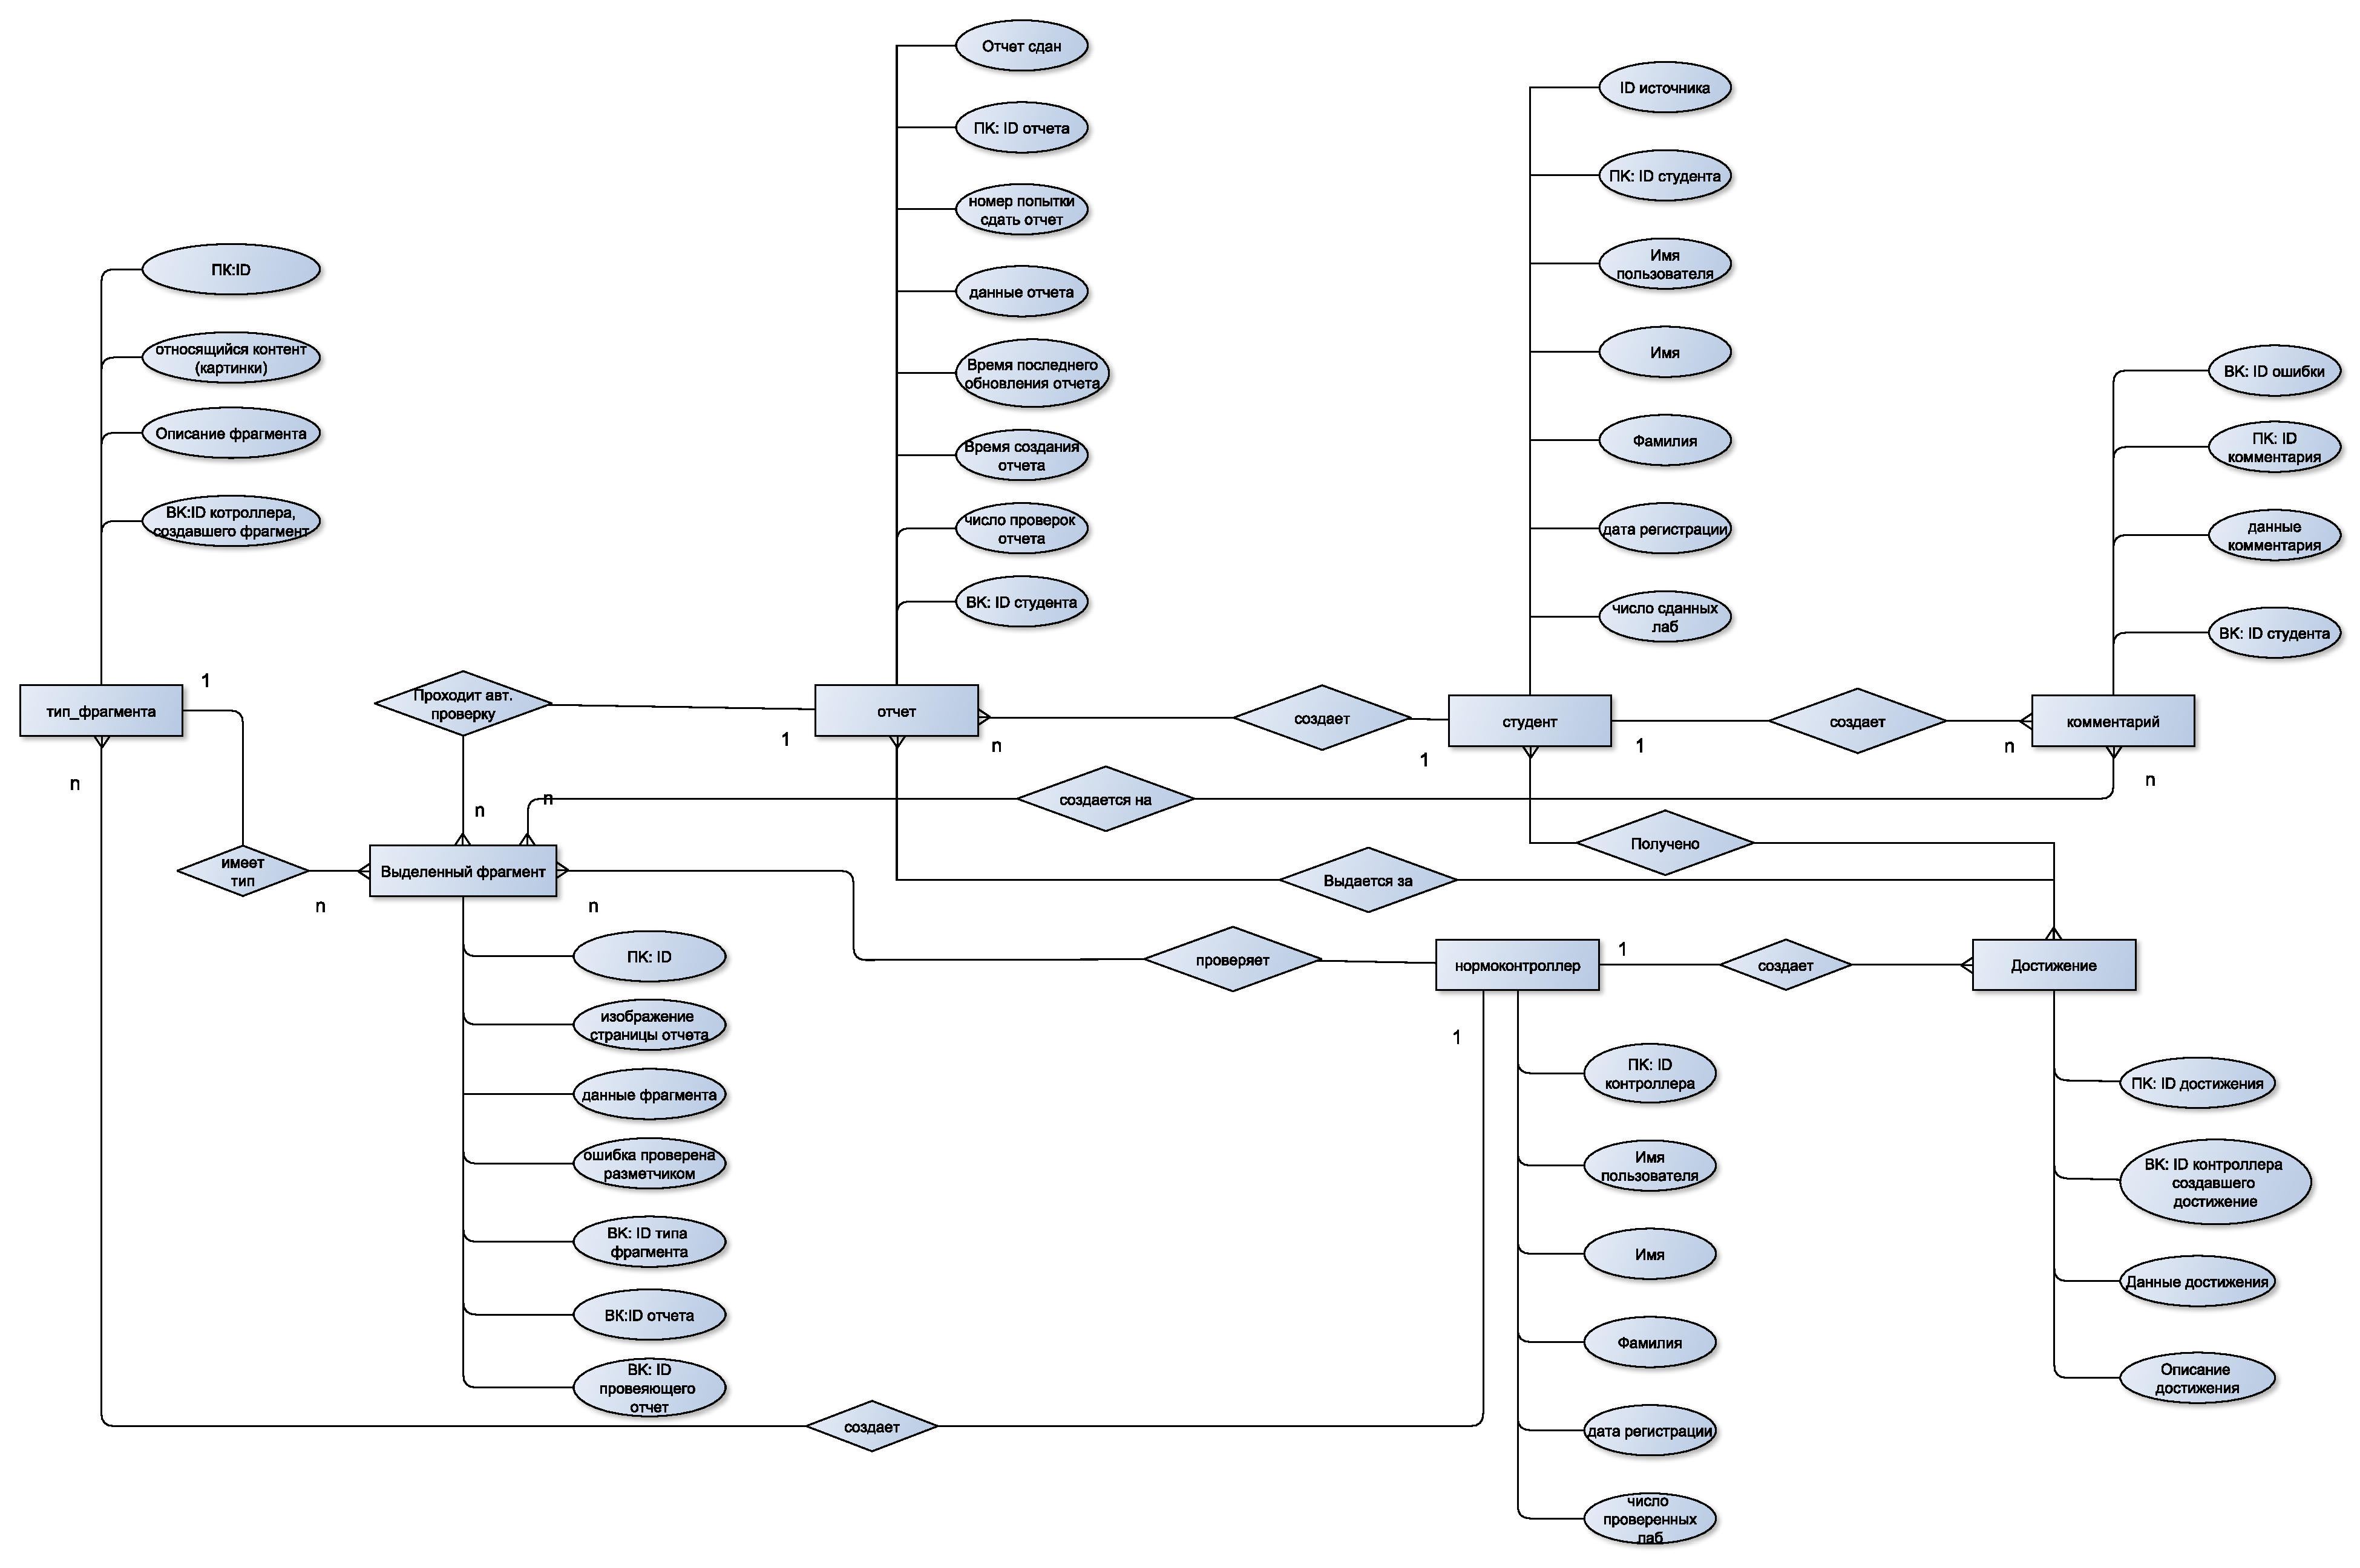
\includegraphics[width=\textheight]{./inc/img/ER_RU.pdf}
	\caption{Диаграмма сущность---связь}
	\label{img:ER_RU}
\end{sidewaysfigure}

\section{Формализация пользователей}
При анализе предметной области были выделены следующие роли в системе:
\begin{itemize}
	\item гость --- данная роль представляет не авторизованного пользователя, соответственно он может авторизоваться и войти в систему;
	\item студент --- данная роль позволяет создавать комментарии к отчетам,
	просматривать отправленные документы и ошибки в них;
	\item нормоконтроллер --- данная роль позволяет создавать типы разметок, разметки элементов отчета, просматривать отправленные документы и ошибки в них, а также создавать, удалять, модифицировать достижения и создавать комментарии;
	\item админ --- возможности данной роли аналогичны роли нормоконтроллера, однако данная роль также позволяет удалять типы элементов отчета и изменять роль пользователей (со студента на нормоконтроллера и наборот).
\end{itemize}


Для описания сценариев взаимодействия пользователей с системой была создана диаграмма прецедентов, представленная на рисунке~\ref{img:BD_use_cases}.

\includeimage
{BD_use_cases} % Имя файла без расширения (файл должен быть расположен в директории inc/img/)
{f} % Обтекание (без обтекания)
{H} % Положение рисунка (см. figure из пакета float)
{1\textwidth} % Ширина рисунка
{Диаграмма прецедентов} % Подпись рисунка


\section{Анализ существующих баз данных}
База данных —-- это некоторый набор перманентных (постоянно хранимых) данных, используемых прикладными программными системами какого-либо предприятия~\cite{williams-db}.

Между физической базой данных (т.е. данными, которые реально хранятся на компьютере) и пользователями системы располагается уровень программного
обеспечения, который можно называть по-разному: диспетчер базы данных (database 
manager), сервер базы данных (database server) или, что более привычно, система управления базами данных, СУБД (DataBase Management System — DBMS).
Основная задача СУБД --- дать пользователю базы данных возможность работать с ней, не вникая во все подробности работы на уровне аппаратного обеспечения~\cite{williams-db}.

Модель данных — это абстрактное, самодостаточное, логическое определение объектов, операторов и прочих элементов, в совокупности составляющих абстрактную машину доступа к данным, с которой взаимодействует пользователь~\cite{williams-db}.
Рассмотрим классификацию баз данных по различным моделям данных:
\begin{itemize}
	\item дореляционные;
	\item реляционные;
	\item постреляционные.
\end{itemize}

\subsection{Дореляционные модели}
Дореляционные системы можно разделить на три большие категории:
\begin{itemize}
	\item системы с инвертированными списками;
	\item иерархические;
	\item сетевые~\cite{williams-db}.
\end{itemize}
Иерархическая база данных представляется множеством 
деревьев: в вершинах дерева помещаются записи, состоящие из поименованных 
полей и представляющие экземпляры некоторого объекта предметной области. 
Записи связаны строго иерархическими отношениями --- у записи-<<потомка>> не 
должно быть более одной записи-<<предка>>~\cite{wolf-db}.

Сетевая модель данных представляет собой логическую модель данных, которая расширяет иерархический подход. В иерархических структурах каждая запись-потомок имеет ровно одного предка, в то время как в сетевой структуре данных потомок может иметь несколько предков~\cite{wolf-db}.


Инвертированный список - это способ организации данных, который позволяет быстро находить записи по определенному значению, в общем случае он состоит из 3 уровней~\cite{inverted-lists}. 

Первый уровень это файл или часть файла, где хранятся все уникальные упорядоченные значения вторичных ключей.Для каждого значения вторичного ключа есть ссылка на первый блок в цепочке блоков, содержащих номера записей с этим значением вторичного ключа. Каждый блок представляет собой список номеров записей~\cite{inverted-lists}.

Второй уровень состоит из цепочки блоков, содержащих номера записей с идентичным значением вторичного ключа. Блоки второго уровня также упорядочены по значениям вторичного ключа~\cite{inverted-lists}.

Последним уровнем является сам файл данных, где хранятся данные, для быстрого поиска записей доступ к ним осуществляется через блоки второго уровня~\cite{inverted-lists}.

Поиск в данной структуре осуществляется следующим образом: система просматривает первый уровень инвертированного списка и ищет заданное значение вторичного ключа. Когда значение найдено, система получает ссылку на первый блок на втором уровне. Затем система просматривает блоки второго уровня, пока не найдет блок с нужным значением вторичного ключа. После чего система использует номера записей из найденного блока, чтобы загрузить содержимое соответствующих записей в рабочую область пользователя.~\cite{inverted-lists}.




\subsection{Реляционные модели}
Реляционная база данных — это такая база данных, которая воспринимается ее пользователями как множество переменных (т.е. переменных отношения), значениями которых являются отношения или, менее формально, таблицы~\cite{williams-db}.

Реляционная система, поддерживает реляционные базы данных и осуществляет операции над ними, включая RESTRICT (также известную как выборка или англ. SELECT), проекцию (англ. PROJECT) и соединение (англ. JOIN). Эти и подобные операции реляционной алгебры выполняются на уровне множеств~\cite{williams-db}.

\subsection{Постреляционные модели}
Современный (постреляционный) этап развития связан с использованием объектно-ориентированных технологий разработки программных систем и созданием СУБД нового поколения, унаследовавших все лучшее от дореляционных и реляционных систем. Постреляционные СУБД поддерживают 
объектные и объектно-реляционные модели данных и обеспечивают разработчикам возможность использовать объектно-ориентированные языки программирования, что дает таким системам технологические преимущества по сравнению с реляционными СУБД~\cite{wolf-db}.

\subsection{Хранение временных рядов}
Отдельно стоит отметить набирающие популярность СУБД временных рядов. Временные ряды (англ. Time series) --- это данные, 
претерпевающие некоторые изменения с течением 
времени, и фиксируемые в конкретные промежутки 
времени. Данные СУБД оптимизированы под частую запись данных и скорость получения доступа к данным не настолько сильно зависит от числа хранимых данных, что характерно для реляционных баз данных, скорость работы которых уменьшается ввиду необходимости индексирования новых элементов. Однако во временных СУБД отсутствует механизм изменения записанных значений, так как считается что записанные метрики (данные) являются фактом в прошлом~\cite{time_db}.

\section*{Вывод}
В данном разделе были описаны основные ошибки студентов в отчетах по лабораторным работам, были выделены участники процесса приема лабораторных работ, формализован процесс приема лабораторных работ, а также рассмотрены существующие средства автоматизации проверки работ на соответствие стандартам, были формализованы требования к базе данных и приложению. 

